% ╔══════════════════════════════════════════════════════════════════════╗
%  Technical Report — Plague Containment
%  Computer Sciences I — 2026-I  |  Team 16
%  Universidad Distrital Francisco José de Caldas
% ╚══════════════════════════════════════════════════════════════════════╝
\documentclass[12pt, a4paper]{article}

% ── Packages ──────────────────────────────────────────────────────────
\usepackage[T1]{fontenc}
\usepackage[utf8]{inputenc}
\usepackage{geometry}
\geometry{margin=2.54cm}
\usepackage{setspace}
\onehalfspacing
\usepackage{titlesec}
\usepackage{fancyhdr}
\usepackage{graphicx}
\usepackage{amsmath,amssymb}
\usepackage{algorithm}
\usepackage{algorithmic}
\usepackage{listings}
\usepackage{xcolor}
\usepackage{tikz}
\usepackage{tabularx}
\usepackage{booktabs}
\usepackage{array}
\usepackage{hyperref}
\usepackage{tocloft}
\usepackage{placeins}
\usepackage{caption}
\usetikzlibrary{positioning, arrows.meta, shapes.geometric, shadows}

\renewcommand{\algorithmicrequire}{\textbf{Input:}}
\renewcommand{\algorithmicensure}{\textbf{Output:}}

% ── Hyperref setup ────────────────────────────────────────────────────
\hypersetup{
  colorlinks = true,
  linkcolor  = blue!60!black,
  citecolor  = blue!60!black,
  urlcolor   = blue!60!black
}

% ── JSON listing style ────────────────────────────────────────────────
\definecolor{jsonkey}{RGB}{163,21,21}
\definecolor{jsonstring}{RGB}{0,128,0}
\definecolor{jsonnumber}{RGB}{0,0,205}
\lstdefinelanguage{json}{
  basicstyle=\ttfamily\small,
  columns=fullflexible,
  showstringspaces=false,
  commentstyle=\color{gray},
  string=[s]{"}{"},
  stringstyle=\color{jsonstring},
  literate=
    *{0}{{{\color{jsonnumber}0}}}{1}
     {1}{{{\color{jsonnumber}1}}}{1}
     {2}{{{\color{jsonnumber}2}}}{1}
     {3}{{{\color{jsonnumber}3}}}{1}
     {4}{{{\color{jsonnumber}4}}}{1}
     {5}{{{\color{jsonnumber}5}}}{1}
     {6}{{{\color{jsonnumber}6}}}{1}
     {7}{{{\color{jsonnumber}7}}}{1}
     {8}{{{\color{jsonnumber}8}}}{1}
     {9}{{{\color{jsonnumber}9}}}{1}
     {:}{{{\color{jsonkey}{:}}}}{1}
     {,}{{{\color{black}{,}}}}{1}
     {\{}{{{\color{black}{\{}}}}{1}
     {\}}{{{\color{black}{\}}}}}{1}
     {[}{{{\color{black}{[}}}}{1}
     {]}{{{\color{black}{]}}}}{1},
}

% ── Header / Footer ───────────────────────────────────────────────────
\pagestyle{fancy}
\fancyhf{}
\rhead{\small Technical Report --- Plague Containment}
\lhead{\small Computer Sciences I, 2026-I}
\cfoot{\thepage}
\renewcommand{\headrulewidth}{0.4pt}

% ── Section formatting ────────────────────────────────────────────────
\titleformat{\section}{\large\bfseries}{}{0em}{\thesection.\quad}
\titleformat{\subsection}{\normalsize\bfseries}{}{0em}{\thesubsection\quad}

% ══════════════════════════════════════════════════════════════════════
\begin{document}

% ── Title Page ────────────────────────────────────────────────────────
\begin{titlepage}
  \centering
  \vspace*{1.5cm}

  {\Large \textbf{Universidad Distrital Francisco Jos\'{e} de Caldas}}\\[0.4cm]
  {\large Computer Engineering Program}\\[0.4cm]
  {\large Computer Sciences I --- 2026-I}\\[2.0cm]

  \rule{\linewidth}{1.5pt}\\[0.4cm]
  {\Huge \textbf{Plague Containment}}\\[0.3cm]
  {\large \textit{Technical Report --- Checkpoint Week 8}}\\[0.2cm]
  \rule{\linewidth}{1.5pt}\\[2.0cm]

  \begin{tabular}{ll}
    \textbf{Team 16} & \\[0.3cm]
    Nelson David Molina Ramos         & \texttt{Data Structures (C++)}\\[0.2cm]
    Brayan Estiven Aguirre Aristizabal & \texttt{Algorithms (Python)}\\[0.2cm]
    Juan Sneyder M\'{e}ndez Gil        & \texttt{Interface \& Integration}\\
  \end{tabular}

  \vfill
  {\large Bogot\'{a}, Colombia\\[0.2cm] \today}
\end{titlepage}

% ── Table of Contents ─────────────────────────────────────────────────
\newpage
\tableofcontents

% ── List of Figures ───────────────────────────────────────────────────
\newpage
\listoffigures
\listoftables

% ══════════════════════════════════════════════════════════════════════
\newpage
\section{Abstract}

Plague Containment is a turn-based strategy game designed as part of the
Computer Sciences~I course project at Universidad Distrital Francisco
Jos\'{e} de Caldas. The game models a city as an $8\times8$ grid of
districts, each carrying an infection risk level, and challenges the player
to stop a spreading plague using two algorithmic tools: a greedy vaccination
advisor that always targets the highest-risk unprotected district on the
infection border, and a backtracking quarantine planner that searches for a
ring of districts enclosing the infected zone without isolating any healthy
area. This report presents the complete design of the system, including the
city model, the pseudo-code of both algorithms, the three-layer architecture
(C++ engine, Python algorithms, Pygame interface), the JSON communication
schema that bridges all layers, and the wireframe of the game interface. No
implementation has been completed at this stage; the next steps are to code
the algorithms, build the interface, and develop the C++ engine.

% ══════════════════════════════════════════════════════════════════════
\newpage
\section{Introduction}

Epidemic spread is a well-studied problem both in epidemiology and in
computer science. Models that represent populations as graphs or grids have
been used to simulate the progression of infections and to evaluate
containment strategies~\cite{pastor2015epidemic}. Algorithmic approaches
such as greedy heuristics and exhaustive search with backtracking are
fundamental tools for solving optimization and constraint-satisfaction
problems of this kind, as described in standard references on
algorithms~\cite{cormen2009introduction} and artificial
intelligence~\cite{russell2020artificial}.

Plague Containment applies these ideas in the context of a video game.
The player is placed in charge of a city represented as an $8\times8$ grid
of districts. Each district carries an infection risk level, and the plague
spreads every turn to neighboring districts. The player has two tools at
their disposal: they may vaccinate a district to make it permanently immune,
or they may trigger a quarantine perimeter that isolates the infected zone.
Two algorithms assist the player: a greedy advisor that recommends the
single most dangerous unprotected neighbor of the infected zone, and a
backtracking planner that automatically finds a valid quarantine ring while
guaranteeing that no healthy district becomes disconnected from the rest of
the city.

The goal of this report is to document the full design of the game for
the Week~8 checkpoint. It covers the city model, the algorithmic design and
pseudo-code, the system architecture, the JSON communication schema, and the
interface wireframe. Implementation of the system is planned as the next
phase of the project.

% ══════════════════════════════════════════════════════════════════════
\section{Literature Review}

The design of Plague Containment draws on three established areas of
computer science and mathematics.

Epidemic modeling on networks and grids has a long history in applied
mathematics. Pastor-Satorras et al.~\cite{pastor2015epidemic} provide a
comprehensive review of epidemic processes on complex networks, showing how
the local connectivity of a node directly influences how quickly an
infection spreads to its neighbors. This finding motivates the risk-level
model used in Plague Containment: districts with higher risk values represent
nodes that are more likely to propagate the infection, making them the
priority targets for the greedy vaccination strategy.

Greedy algorithms are covered extensively in Cormen et
al.~\cite{cormen2009introduction}, which establishes that a greedy approach
is appropriate when a locally optimal choice at each step leads to a
globally acceptable result. In the vaccination problem, the immediate danger
at each turn comes from the unprotected district with the highest risk on
the infection border; targeting that district first reduces the most urgent
threat and is a natural application of the greedy principle.

Backtracking search is presented by both Cormen et
al.~\cite{cormen2009introduction} and Russell and
Norvig~\cite{russell2020artificial} as the standard technique for
constraint-satisfaction problems in which a partial solution must be
extended step by step, with the ability to undo choices that violate
constraints. The quarantine problem requires simultaneous satisfaction of
two constraints --- full enclosure of the infected zone and preservation of
the connectivity of the healthy city --- which cannot be guaranteed by a
greedy selection, making backtracking the appropriate algorithmic choice.

% ══════════════════════════════════════════════════════════════════════
\section{Objectives}

The main goal of this project is to design and implement a playable,
turn-based strategy game that demonstrates the practical application of
greedy and backtracking algorithms in the context of epidemic containment.

The specific objectives for the Week~8 checkpoint are:

\begin{enumerate}
  \item Define a formal model of the city grid, including district states,
        risk levels, and plague spread rules.
  \item Design and express in pseudo-code a greedy algorithm that
        recommends the best district to vaccinate each turn.
  \item Design and express in pseudo-code a backtracking algorithm that
        finds a valid quarantine perimeter around the infected zone while
        preserving city connectivity.
  \item Define a three-layer system architecture and a JSON communication
        schema that allows a C++ engine, a Python algorithm module, and a
        Pygame interface to exchange data without direct language bindings.
  \item Produce a wireframe of the game interface that reflects the
        information provided by both the engine and the algorithms.
\end{enumerate}

% ══════════════════════════════════════════════════════════════════════
\section{Scope}

This report covers the design phase of the Plague Containment project
(Week~8 checkpoint). It includes the city model, algorithmic design,
system architecture, JSON schema, and interface wireframe. It does not
include working source code, test results, or performance measurements,
as those belong to subsequent checkpoints. The game is intended to run
locally on a desktop machine and is designed for a single player.

The grid is fixed at $8\times8$ districts. Risk levels are integers from
1 to 10 assigned once at game start and do not change. The game ends when
either all infected districts are contained (player wins) or the plague
spreads to more than a predefined threshold of districts (player loses).

% ══════════════════════════════════════════════════════════════════════
\section{Assumptions}

The following assumptions were made during the design of the system:

\begin{enumerate}
  \item Adjacency is defined as sharing a side (4-connectivity: up, down,
        left, right). Diagonal neighbors are not considered adjacent.
  \item The plague spreads with a non-zero probability to every unprotected
        healthy neighbor of every infected district at the end of each turn.
        The exact probability is a design parameter to be set during
        implementation.
  \item A district in the \emph{quarantined} or \emph{vaccinated} state
        completely blocks plague spread; no probabilistic transmission occurs
        across those borders.
  \item The backtracking algorithm operates on the set of healthy districts
        that border the infected zone. It is assumed that this set is finite
        and small enough for exhaustive search within the response time of
        a single game turn.
  \item JSON file I/O is fast enough relative to the game's turn duration
        that it does not create noticeable latency for the player.
  \item All three system components (C++ engine, Python algorithms, Pygame
        interface) run on the same local machine and share access to the
        same filesystem directory.
\end{enumerate}

% ══════════════════════════════════════════════════════════════════════
\section{Limitations}

The current design has several known limitations:

\begin{enumerate}
  \item The backtracking quarantine algorithm explores all possible subsets
        of border districts. In the worst case its running time is
        exponential in the number of border districts. For a densely
        infected grid the algorithm could be slow, but in practice the
        border set is small and the constraint checks prune most branches
        early.
  \item The JSON bridge introduces a file I/O overhead on every turn. For
        a turn-based game this overhead is acceptable, but the design is
        not suitable for real-time applications.
  \item The current design does not include a multiplayer mode, difficulty
        scaling beyond risk level assignment, or an AI opponent.
  \item The wireframe presented in this report is a design prototype. The
        final visual style, color palette, and layout may change during
        implementation.
  \item No formal risk analysis has been performed on the probability model
        for plague spread. The spread mechanics described here are
        conceptual and will require calibration during testing.
\end{enumerate}

% ══════════════════════════════════════════════════════════════════════
\section{Methodology}

\subsection{City Grid Model}

The city is represented as an $8\times8$ grid of districts. Each cell in
the grid corresponds to one district, and two districts are considered
neighbors if they share a side (up, down, left, or right). Every district
is always in exactly one of the four states described in
Table~\ref{tab:states}.

\begin{table}[ht]
\centering
\caption{District states and their meaning in the game.}
\label{tab:states}
\begin{tabularx}{\linewidth}{|l|X|}
\hline
\textbf{State} & \textbf{Description} \\
\hline
Healthy     & Not yet affected by the plague. Can become infected. \\
\hline
Infected    & Currently carrying the plague; attempts to spread to
              healthy neighbors each turn. \\
\hline
Vaccinated  & Permanently immunized by the player. Cannot become
              infected and blocks spread. \\
\hline
Quarantined & Placed under lockdown by the backtracking planner to form
              the containment perimeter. Blocks spread. \\
\hline
\end{tabularx}
\end{table}

Each district also carries a \emph{risk level}, which is a whole number
between 1 and 10 assigned at the start of the game. A higher risk level
indicates greater vulnerability to infection, for example due to high
population density or poor sanitation. The risk level does not change
during the game. Figure~\ref{fig:grid} shows an example state of the
grid mid-game.

\begin{figure}[ht]
  \centering
  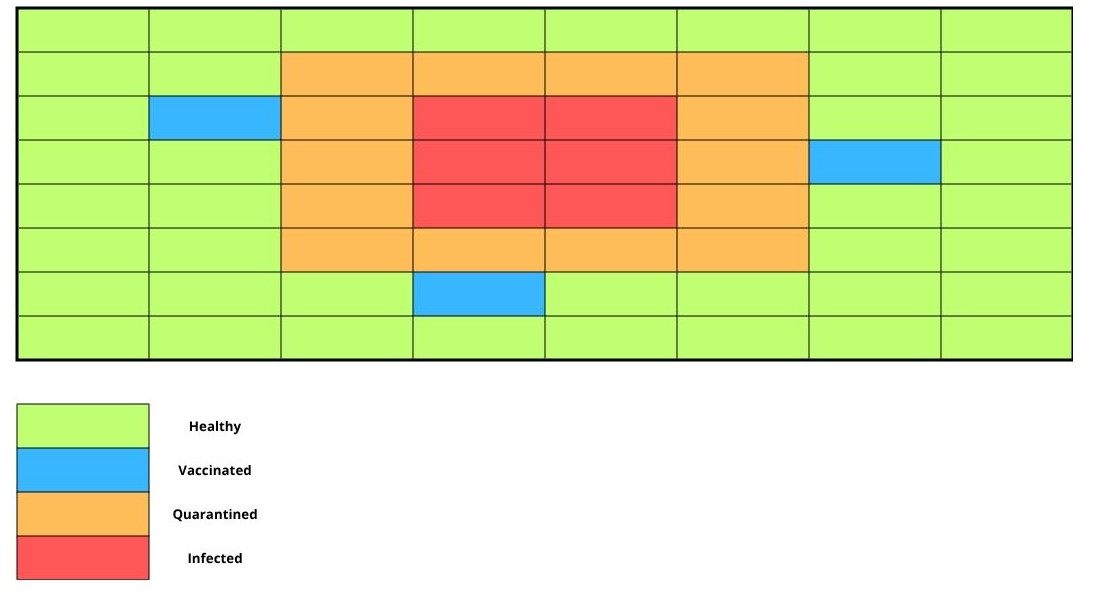
\includegraphics[width=0.5\textwidth]{f1.jpg}
  \caption{Example of the game grid mid-game. Green cells are vaccinated,
           red cells are infected, blue cells are quarantined, and yellow-green
           cells are healthy.}
  \label{fig:grid}
\end{figure}

At the end of each turn the plague attempts to spread: for every infected
district, each of its healthy neighbors has a chance of becoming infected.
Districts in the vaccinated or quarantined state block spread entirely.

\subsection{Greedy Vaccination Algorithm}

The greedy algorithm helps the player decide which district to vaccinate
each turn. It scans every healthy district that directly borders an infected
one and recommends the district with the highest risk level. The rationale
is straightforward: the most dangerous unprotected neighbor on the infection
border is the one most likely to spread the plague further if left unprotected,
so targeting it first provides the best immediate reduction of risk.

Greedy algorithms are appropriate when a locally optimal decision at each
step leads to a globally acceptable outcome. In the vaccination problem the
immediate threat is always concentrated in the border district with the
highest risk, so a local scan of the border is sufficient to make a useful
recommendation without looking ahead across multiple turns. Algorithm~\ref{alg:greedy}
shows the complete pseudo-code.

\begin{algorithm}[ht]
\caption{Greedy Vaccination}
\label{alg:greedy}
\begin{algorithmic}[1]
\REQUIRE The game grid with all district states and risk levels
\ENSURE The best district to vaccinate this turn, or \textsc{None}
\STATE $\mathit{candidates} \leftarrow$ empty list
\FOR{each infected district $d$ on the grid}
  \FOR{each neighbor $n$ of $d$}
    \IF{$n$ is \textsc{Healthy}}
      \STATE add $n$ to $\mathit{candidates}$ (avoid duplicates)
    \ENDIF
  \ENDFOR
\ENDFOR
\IF{$\mathit{candidates}$ is empty}
  \RETURN \textsc{None}
\ENDIF
\STATE $\mathit{best} \leftarrow$ first district in $\mathit{candidates}$
\FOR{each district $c$ in $\mathit{candidates}$}
  \IF{$c.\mathit{risk} > \mathit{best}.\mathit{risk}$}
    \STATE $\mathit{best} \leftarrow c$
  \ENDIF
\ENDFOR
\STATE mark $\mathit{best}$ as \textsc{Vaccinated}
\RETURN $\mathit{best}$
\end{algorithmic}
\end{algorithm}

\subsection{Backtracking Quarantine Algorithm}

The backtracking algorithm finds a set of healthy districts to quarantine
so that the infected zone is completely enclosed. The solution must satisfy
two conditions simultaneously:

\begin{enumerate}
  \item \textbf{Full enclosure.} Every infected district must be completely
        surrounded; none of its neighbors may remain a free healthy district.
  \item \textbf{No isolation.} After quarantine districts are placed, every
        remaining healthy district must still be reachable from the rest of
        the healthy city. No healthy area may become a disconnected island.
\end{enumerate}

A greedy approach is not suitable here because a locally reasonable choice
--- for example, quarantining a district that appears necessary to close the
perimeter --- can accidentally cut a healthy neighborhood off from the rest
of the city. Backtracking allows the algorithm to try a quarantine placement,
verify both conditions, and undo the placement if either condition is
violated, then explore the alternative of skipping that district, until a
valid complete solution is found or all possibilities are exhausted.

Algorithm~\ref{alg:bt_main} is the entry point, and
Algorithm~\ref{alg:bt_worker} is the recursive function it calls.
\vspace{-10pt}
\begin{algorithm}[ht]
\caption{Backtracking Quarantine --- Entry Point}
\label{alg:bt_main}
\begin{algorithmic}[1]
\REQUIRE The game grid with all district states
\ENSURE A valid quarantine set, or \textsc{None} if impossible
\STATE $\mathit{border} \leftarrow$ all healthy neighbors of infected districts
\STATE $\mathit{quarantine} \leftarrow$ empty set
\STATE $\mathit{success} \leftarrow$
       \textsc{Search}($\mathit{border}$, index $0$, $\mathit{quarantine}$)
\IF{$\mathit{success}$}
  \RETURN $\mathit{quarantine}$
\ELSE
  \RETURN \textsc{None}
\ENDIF
\end{algorithmic}
\end{algorithm}
\vspace{-25pt}
\begin{algorithm}[ht]
\caption{Search --- Recursive Backtracking Step}
\label{alg:bt_worker}
\begin{algorithmic}[1]
\REQUIRE Border district list, current index $i$,
         partial quarantine set $\mathit{quarantine}$
\ENSURE \textsc{True} if a complete valid quarantine was found,
        \textsc{False} otherwise
\IF{infected zone is fully enclosed by $\mathit{quarantine}$}
  \RETURN \textsc{True}
\ENDIF
\IF{no more border districts to try}
  \RETURN \textsc{False}
\ENDIF
\STATE $d \leftarrow \mathit{border}[i]$
\COMMENT{--- Option A: quarantine district $d$ ---}
\STATE add $d$ to $\mathit{quarantine}$
\STATE temporarily mark $d$ as \textsc{Quarantined} on the grid
\IF{remaining healthy districts are still all connected}
  \IF{\textsc{Search}($\mathit{border}$, $i+1$, $\mathit{quarantine}$)}
    \RETURN \textsc{True}
  \ENDIF
\ENDIF
\COMMENT{--- Backtrack: undo quarantine of $d$ ---}
\STATE remove $d$ from $\mathit{quarantine}$
\STATE restore $d$ to \textsc{Healthy} on the grid
\COMMENT{--- Option B: skip district $d$ ---}
\IF{\textsc{Search}($\mathit{border}$, $i+1$, $\mathit{quarantine}$)}
  \RETURN \textsc{True}
\ENDIF
\RETURN \textsc{False}
\end{algorithmic}
\end{algorithm}

\subsection{Game Turn Structure}

The greedy and backtracking algorithms serve different roles within a single
turn. Figure~\ref{fig:loop} shows the sequence of events. The greedy
algorithm runs at the start of the turn, before the player acts, so that
the recommendation is based on the current grid state. The backtracking
planner runs after the plague spreads, so that the quarantine perimeter
it computes always reflects the most up-to-date infection state.

\begin{figure}[H]
\centering
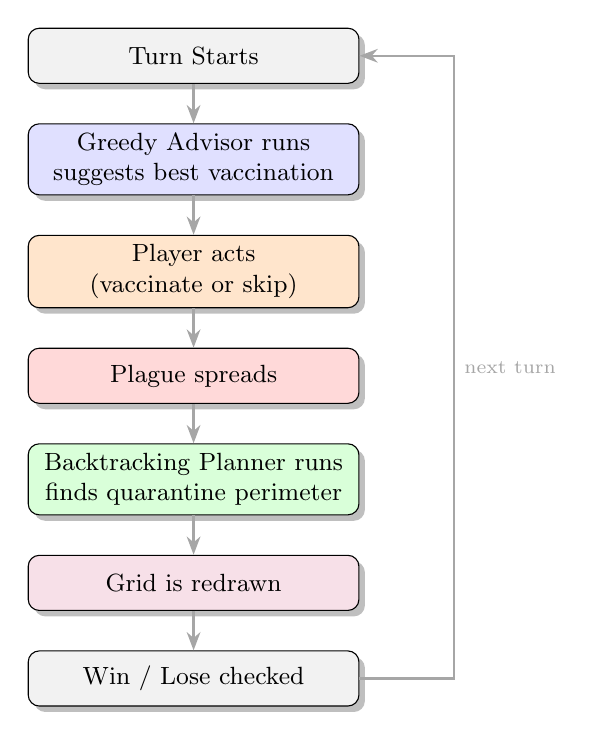
\begin{tikzpicture}[
  box/.style={draw, rounded corners=4pt, minimum width=4.2cm,
              minimum height=0.70cm, align=center, font=\small,
              fill=white, drop shadow},
  arr/.style={-Stealth, thick, gray!70}
]
  \node[box, fill=gray!10]   (start)  {Turn Starts};
  \node[box, fill=blue!12,   below=0.5cm of start]  (greedy)
    {Greedy Advisor runs\\suggests best vaccination};
  \node[box, fill=orange!20, below=0.5cm of greedy] (player)
    {Player acts\\(vaccinate or skip)};
  \node[box, fill=red!15,    below=0.5cm of player] (spread)
    {Plague spreads};
  \node[box, fill=green!15,  below=0.5cm of spread] (bt)
    {Backtracking Planner runs\\finds quarantine perimeter};
  \node[box, fill=purple!12, below=0.5cm of bt]     (render)
    {Grid is redrawn};
  \node[box, fill=gray!10,   below=0.5cm of render] (check)
    {Win / Lose checked};
  \draw[arr] (start)  -- (greedy);
  \draw[arr] (greedy) -- (player);
  \draw[arr] (player) -- (spread);
  \draw[arr] (spread) -- (bt);
  \draw[arr] (bt)     -- (render);
  \draw[arr] (render) -- (check);
  \draw[arr] (check.east) -- ++(1.2,0) |- (start.east)
    node[pos=0.25, right, font=\scriptsize] {next turn};
\end{tikzpicture}
\caption{Sequence of events inside one game turn.}
\label{fig:loop}
\end{figure}

\subsection{System Architecture}

Plague Containment is organized in three independent layers, each
implemented in a different language. The C++ engine manages the core game
state, including a linked list that tracks the infection chain in insertion
order and an AVL tree that indexes districts by risk level for fast lookup.
The Python module implements both algorithms. The Pygame interface renders
the grid, displays the algorithm suggestions, and handles player input.
Table~\ref{tab:components} summarizes the responsibility of each layer.

\begin{table}[ht]
\centering
\caption{Responsibility of each system component.}
\label{tab:components}
\begin{tabularx}{\linewidth}{|l|l|X|}
\hline
\textbf{Layer} & \textbf{Language} & \textbf{Responsibilities} \\
\hline
Engine     & C++            & Maintain the infection chain (linked list) and
                              district risk index (AVL tree). Update plague
                              spread each turn. Write the updated game state
                              to \texttt{state.json}. \\
\hline
Algorithms & Python         & Read the game state from \texttt{state.json}.
                              Run the greedy advisor and the backtracking
                              planner. Write results to
                              \texttt{result.json}. \\
\hline
Interface  & Python/Pygame  & Read \texttt{state.json} and
                              \texttt{result.json}. Render the grid,
                              highlights, and HUD. Capture player input and
                              write the chosen action to
                              \texttt{action.json}. \\
\hline
\end{tabularx}
\end{table}

The three layers do not call each other directly. Instead they communicate
through three shared JSON files that act as a language-neutral bridge. This
design avoids the complexity of cross-language bindings and makes debugging
straightforward, since any team member can open the JSON files at any point
and inspect the complete game state.

Figure~\ref{fig:dataflow} shows the data flow among the three layers during
a single turn.

\begin{figure}[ht]
\centering
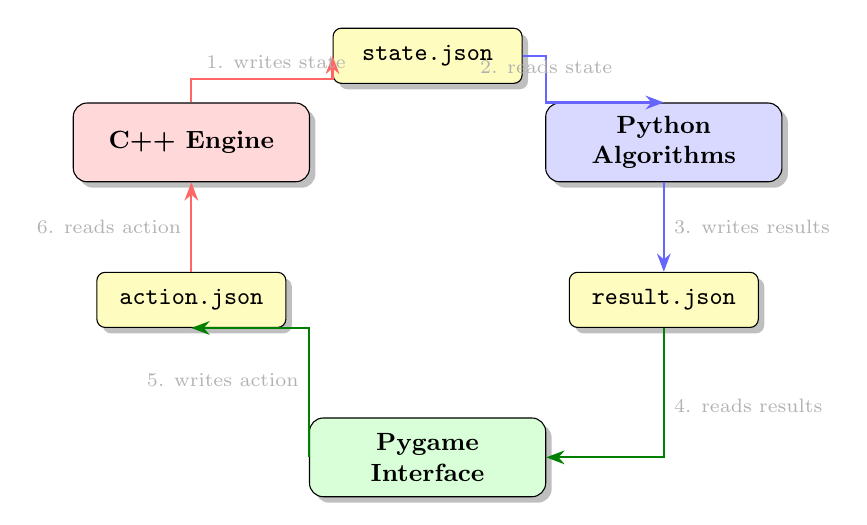
\begin{tikzpicture}[
  component/.style={draw, rounded corners=5pt, minimum width=3.0cm,
              minimum height=1.0cm, align=center, font=\small\bfseries,
              drop shadow},
  jsonbox/.style={draw, rounded corners=3pt, minimum width=2.4cm,
              minimum height=0.7cm, align=center, font=\small,
              fill=yellow!25, drop shadow},
  arr/.style={-Stealth, thick},
  note/.style={font=\scriptsize, text=gray!60}
]
  \node[component, fill=red!15]    (cpp)  at (0, 0)      {C++ Engine};
  \node[component, fill=blue!15]   (py)   at (6.0, 0)    {Python\\Algorithms};
  \node[component, fill=green!15]  (ui)   at (3.0, -4.0) {Pygame\\Interface};
  \node[jsonbox] (json1) at (3.0,  1.1)  {\texttt{state.json}};
  \node[jsonbox] (json2) at (6.0, -2.0)  {\texttt{result.json}};
  \node[jsonbox] (json3) at (0,   -2.0)  {\texttt{action.json}};
  \draw[arr, red!60]   (cpp.north) -- ++(0,0.3) -| (json1.west)
    node[pos=0.3, above, note] {1. writes state};
  \draw[arr, blue!60]  (json1.east) -- ++(0.3,0) |- (py.north)
    node[pos=0.3, above, note] {2. reads state};
  \draw[arr, blue!60]  (py.south) -- (json2.north)
    node[midway, right, note] {3. writes results};
  \draw[arr, green!50!black] (json2.south) |- (ui.east)
    node[pos=0.3, right, note] {4. reads results};
  \draw[arr, green!50!black] (ui.west) |- (json3.south)
    node[pos=0.3, left, note] {5. writes action};
  \draw[arr, red!60]   (json3.north) -- (cpp.south)
    node[midway, left, note] {6. reads action};
\end{tikzpicture}
\caption{Data flow between the three system components through JSON files.
         Numbers indicate the order of operations within one turn.}
\label{fig:dataflow}
\end{figure}

\subsection{JSON Schema Design}

Three JSON files mediate all inter-component communication. Each file has a
clearly defined structure and a single writer and one or more readers.

\textbf{\texttt{state.json}} is written by the C++ engine at the start of
each turn. It contains the complete snapshot of the grid, including the
state and risk level of every district, the infection chain in insertion
order (mirroring the C++ linked list), and precomputed counters for the
interface HUD. Listing~\ref{lst:state} shows an example.

\begin{lstlisting}[language=json, frame=single,
  caption={Example \texttt{state.json} at turn 3.},
  label={lst:state}]
{
  "turn": 3,
  "grid_size": 8,
  "districts": [
    { "row": 0, "col": 0, "risk": 5, "state": "healthy"     },
    { "row": 0, "col": 1, "risk": 8, "state": "infected"    },
    { "row": 1, "col": 0, "risk": 3, "state": "vaccinated"  },
    { "row": 1, "col": 1, "risk": 7, "state": "quarantined" }
  ],
  "infection_chain": [
    { "row": 3, "col": 4, "turn_infected": 1 },
    { "row": 3, "col": 5, "turn_infected": 1 },
    { "row": 2, "col": 4, "turn_infected": 2 },
    { "row": 4, "col": 4, "turn_infected": 3 }
  ],
  "stats": {
    "total_infected":    4,
    "total_vaccinated":  6,
    "total_quarantined": 2,
    "total_healthy":    52
  }
}
\end{lstlisting}

\textbf{\texttt{result.json}} is written by the Python algorithm module
after processing the game state. It contains the greedy vaccination
recommendation and the backtracking quarantine plan. If no valid quarantine
exists, the \texttt{found} field is set to \texttt{false} and the
\texttt{districts} array is empty. Listing~\ref{lst:result} shows an example.

\begin{lstlisting}[language=json, frame=single,
  caption={Example \texttt{result.json}.},
  label={lst:result}]
{
  "greedy_recommendation": {
    "row": 2, "col": 5,
    "risk": 9,
    "reason": "highest-risk healthy neighbor"
  },
  "quarantine_plan": {
    "found": true,
    "districts": [
      { "row": 2, "col": 3 },
      { "row": 4, "col": 5 },
      { "row": 5, "col": 4 },
      { "row": 3, "col": 6 }
    ],
    "cost": 4
  }
}
\end{lstlisting}

\textbf{\texttt{action.json}} is written by the Pygame interface when the
player makes a decision. The \texttt{action\_type} field can be
\texttt{"vaccinate"}, \texttt{"quarantine"}, or \texttt{"skip"}.
Listing~\ref{lst:action} shows an example.

\begin{lstlisting}[language=json, frame=single,
  caption={Example \texttt{action.json}.},
  label={lst:action}]
{
  "turn": 3,
  "action_type": "vaccinate",
  "target": { "row": 2, "col": 5 }
}
\end{lstlisting}

\subsection{Interface Design}

The game window is divided into two regions: the main $8\times8$ grid on
the left and an information panel on the right. Each cell displays its risk
level as a number, and distinct colors encode the four district states:
white for healthy, red for infected, green for vaccinated, and purple for
quarantined. The district currently recommended by the greedy advisor is
marked with a yellow border. The side panel shows turn number, district
counts, the greedy suggestion, the quarantine plan status, and three action
buttons (VACCINATE, QUARANTINE, SKIP~TURN). Figures~\ref{fig:wireframe}
and~\ref{fig:wireframe_detail} show the planned layout.

\begin{figure}[ht]
\centering
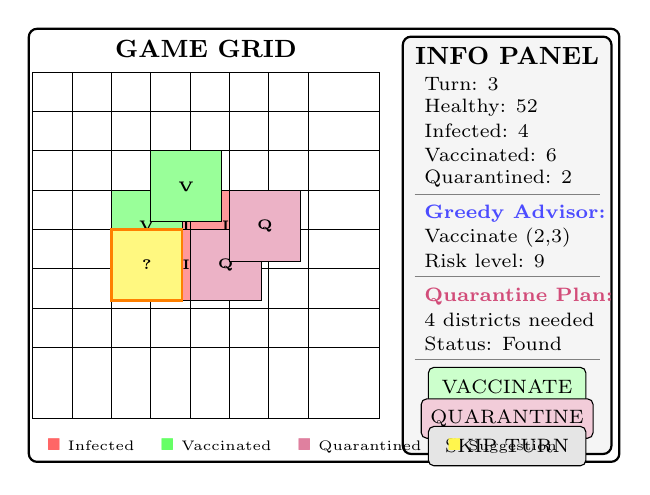
\begin{tikzpicture}[
  scale=0.50,
  cell/.style={draw, minimum size=0.9cm, inner sep=0pt, font=\tiny},
]
  \draw[thick, rounded corners=3pt] (-0.5, -0.5) rectangle (14.5, 10.5);
  \node[font=\small\bfseries] at (4, 10) {GAME GRID};
  \foreach \r in {0,...,7} {
    \foreach \c in {0,...,7} {
      \node[cell, fill=white] at (\c+0.5, 8.5-\r) {};
    }
  }
  \node[cell, fill=red!40]    at (3.5, 5.5) {\textbf{I}};
  \node[cell, fill=red!40]    at (4.5, 5.5) {\textbf{I}};
  \node[cell, fill=red!40]    at (3.5, 4.5) {\textbf{I}};
  \node[cell, fill=green!40]  at (2.5, 5.5) {\textbf{V}};
  \node[cell, fill=green!40]  at (3.5, 6.5) {\textbf{V}};
  \node[cell, fill=purple!30] at (4.5, 4.5) {\textbf{Q}};
  \node[cell, fill=purple!30] at (5.5, 5.5) {\textbf{Q}};
  \node[cell, fill=yellow!50, draw=orange, thick] at (2.5, 4.5) {\textbf{?}};
  \draw[thick, fill=gray!8, rounded corners=3pt]
    (9, -0.3) rectangle (14.3, 10.3);
  \node[font=\small\bfseries] at (11.65, 9.8) {INFO PANEL};
  \node[font=\scriptsize, anchor=west] at (9.3, 9.1) {Turn: 3};
  \node[font=\scriptsize, anchor=west] at (9.3, 8.5) {Healthy: 52};
  \node[font=\scriptsize, anchor=west] at (9.3, 7.9) {Infected: 4};
  \node[font=\scriptsize, anchor=west] at (9.3, 7.3) {Vaccinated: 6};
  \node[font=\scriptsize, anchor=west] at (9.3, 6.7) {Quarantined: 2};
  \draw[gray] (9.3, 6.3) -- (14.0, 6.3);
  \node[font=\scriptsize\bfseries, anchor=west, text=blue!70]
    at (9.3, 5.8) {Greedy Advisor:};
  \node[font=\scriptsize, anchor=west] at (9.3, 5.2) {Vaccinate (2,3)};
  \node[font=\scriptsize, anchor=west] at (9.3, 4.6) {Risk level: 9};
  \draw[gray] (9.3, 4.2) -- (14.0, 4.2);
  \node[font=\scriptsize\bfseries, anchor=west, text=purple!70]
    at (9.3, 3.7) {Quarantine Plan:};
  \node[font=\scriptsize, anchor=west] at (9.3, 3.1) {4 districts needed};
  \node[font=\scriptsize, anchor=west] at (9.3, 2.5) {Status: Found};
  \draw[gray] (9.3, 2.1) -- (14.0, 2.1);
  \node[draw, rounded corners=2pt, fill=green!20, font=\scriptsize,
        minimum width=2cm, minimum height=0.5cm] at (11.65, 1.4)
    {VACCINATE};
  \node[draw, rounded corners=2pt, fill=purple!20, font=\scriptsize,
        minimum width=2cm, minimum height=0.5cm] at (11.65, 0.6)
    {QUARANTINE};
  \node[draw, rounded corners=2pt, fill=gray!20, font=\scriptsize,
        minimum width=2cm, minimum height=0.5cm] at (11.65, -0.1)
    {SKIP TURN};
  \node[font=\tiny, anchor=west] at (-0.3, -0.1) {
    \textcolor{red!60}{$\blacksquare$} Infected \quad
    \textcolor{green!60}{$\blacksquare$} Vaccinated \quad
    \textcolor{purple!50}{$\blacksquare$} Quarantined \quad
    \textcolor{yellow!70}{$\blacksquare$} Suggestion
  };
\end{tikzpicture}
\caption{Basic wireframe of the Pygame interface showing the grid, info
         panel, and action buttons.}
\label{fig:wireframe}
\end{figure}

\begin{figure}[ht]
\centering
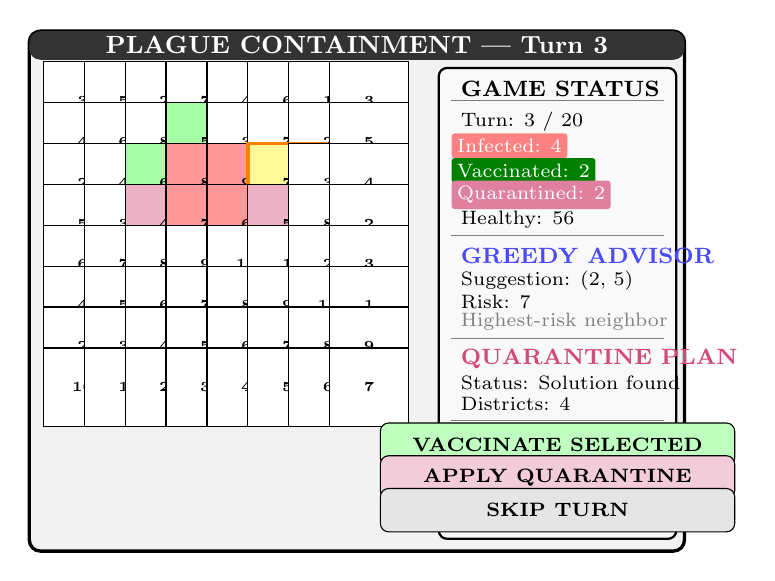
\begin{tikzpicture}[
  scale=0.52,
  cell/.style={draw, minimum size=1.0cm, inner sep=0pt,
               font=\tiny\bfseries},
]
  \draw[very thick, rounded corners=4pt, fill=black!5]
    (-0.8, -1.5) rectangle (15.2, 11.2);
  \fill[black!80, rounded corners=4pt]
    (-0.8, 10.5) rectangle (15.2, 11.2);
  \node[font=\small\bfseries, text=white] at (7.2, 10.85)
    {PLAGUE CONTAINMENT --- Turn 3};
  % Row 0
  \node[cell, fill=white] at (0.5,9.5){3}; \node[cell,fill=white]at(1.5,9.5){5};
  \node[cell, fill=white] at (2.5,9.5){2}; \node[cell,fill=white]at(3.5,9.5){7};
  \node[cell, fill=white] at (4.5,9.5){4}; \node[cell,fill=white]at(5.5,9.5){6};
  \node[cell, fill=white] at (6.5,9.5){1}; \node[cell,fill=white]at(7.5,9.5){3};
  % Row 1
  \node[cell, fill=white]     at (0.5,8.5){4}; \node[cell,fill=white]   at(1.5,8.5){6};
  \node[cell, fill=white]     at (2.5,8.5){8}; \node[cell,fill=green!35]at(3.5,8.5){5};
  \node[cell, fill=white]     at (4.5,8.5){3}; \node[cell,fill=white]   at(5.5,8.5){7};
  \node[cell, fill=white]     at (6.5,8.5){2}; \node[cell,fill=white]   at(7.5,8.5){5};
  % Row 2
  \node[cell, fill=white]     at (0.5,7.5){2}; \node[cell,fill=white]    at(1.5,7.5){4};
  \node[cell, fill=green!35]  at (2.5,7.5){6}; \node[cell,fill=red!40]   at(3.5,7.5){8};
  \node[cell, fill=red!40]    at (4.5,7.5){9};
  \node[cell, fill=yellow!40, draw=orange, very thick] at(5.5,7.5){7};
  \node[cell, fill=white]     at (6.5,7.5){3}; \node[cell,fill=white]    at(7.5,7.5){4};
  % Row 3
  \node[cell, fill=white]     at (0.5,6.5){5}; \node[cell,fill=white]    at(1.5,6.5){3};
  \node[cell, fill=purple!30] at (2.5,6.5){4}; \node[cell,fill=red!40]   at(3.5,6.5){7};
  \node[cell, fill=red!40]    at (4.5,6.5){6}; \node[cell,fill=purple!30]at(5.5,6.5){5};
  \node[cell, fill=white]     at (6.5,6.5){8}; \node[cell,fill=white]    at(7.5,6.5){2};
  % Rows 4-7 (healthy)
  \foreach \r in {4,...,7} {
    \foreach \c in {0,...,7} {
      \pgfmathtruncatemacro{\riskval}{mod(\r*8+\c+3, 10)+1}
      \node[cell, fill=white] at (\c+0.5, 9.5-\r) {\riskval};
    }
  }
  % Side panel
  \draw[thick, fill=gray!5, rounded corners=3pt]
    (9.2, -1.2) rectangle (15.0, 10.3);
  \node[font=\footnotesize\bfseries, anchor=west] at (9.5, 9.8){GAME STATUS};
  \draw[gray] (9.5, 9.5) -- (14.7, 9.5);
  \node[font=\scriptsize, anchor=west] at (9.5, 9.0) {Turn: 3 / 20};
  \node[font=\scriptsize, anchor=west, text=white, fill=red!50,
        rounded corners=1pt, inner sep=2pt] at (9.5, 8.4) { Infected: 4 };
  \node[font=\scriptsize, anchor=west, text=white, fill=green!50!black,
        rounded corners=1pt, inner sep=2pt] at (9.5, 7.8) { Vaccinated: 2 };
  \node[font=\scriptsize, anchor=west, text=white, fill=purple!50,
        rounded corners=1pt, inner sep=2pt] at (9.5, 7.2) { Quarantined: 2 };
  \node[font=\scriptsize, anchor=west] at (9.5, 6.6) {Healthy: 56};
  \draw[gray] (9.5, 6.2) -- (14.7, 6.2);
  \node[font=\footnotesize\bfseries, anchor=west, text=blue!70]
    at (9.5, 5.7) {GREEDY ADVISOR};
  \node[font=\scriptsize, anchor=west] at (9.5, 5.1) {Suggestion: (2, 5)};
  \node[font=\scriptsize, anchor=west] at (9.5, 4.6) {Risk: 7};
  \node[font=\scriptsize, anchor=west, text=gray] at (9.5, 4.1){Highest-risk neighbor};
  \draw[gray] (9.5, 3.7) -- (14.7, 3.7);
  \node[font=\footnotesize\bfseries, anchor=west, text=purple!70]
    at (9.5, 3.2) {QUARANTINE PLAN};
  \node[font=\scriptsize, anchor=west] at (9.5, 2.6){Status: Solution found};
  \node[font=\scriptsize, anchor=west] at (9.5, 2.1) {Districts: 4};
  \draw[gray] (9.5, 1.7) -- (14.7, 1.7);
  \node[draw, rounded corners=3pt, fill=green!25,
        font=\scriptsize\bfseries, minimum width=4.5cm,
        minimum height=0.55cm] at (12.1, 1.1) {VACCINATE SELECTED};
  \node[draw, rounded corners=3pt, fill=purple!20,
        font=\scriptsize\bfseries, minimum width=4.5cm,
        minimum height=0.55cm] at (12.1, 0.3) {APPLY QUARANTINE};
  \node[draw, rounded corners=3pt, fill=gray!20,
        font=\scriptsize\bfseries, minimum width=4.5cm,
        minimum height=0.55cm] at (12.1, -0.5) {SKIP TURN};
\end{tikzpicture}
\caption{Detailed wireframe of the game interface. Each cell shows its risk
         level. Colors encode district states. The yellow-bordered cell marks
         the greedy suggestion.}
\label{fig:wireframe_detail}
\end{figure}

% ══════════════════════════════════════════════════════════════════════
\section{Implementation and Results}

At this checkpoint the project is at the end of the design phase. No
running code has been produced yet; the results of this phase are the
design artifacts described in the Methodology section. This section
summarizes what has been delivered and outlines the work remaining.

Table~\ref{tab:deliverables} lists the design deliverables produced by
each team member for the Week~8 checkpoint.

\begin{table}[ht]
\centering
\caption{Design deliverables per team member at Week~8 checkpoint.}
\label{tab:deliverables}
\begin{tabularx}{\linewidth}{|l|l|X|}
\hline
\textbf{Team Member} & \textbf{Role} & \textbf{Deliverables} \\
\hline
Nelson David Molina Ramos &
Data Structures (C++) &
Design and diagrams of the infection linked list and the district-risk AVL
tree. Explanation of how each structure supports the game engine. \\
\hline
Brayan Estiven Aguirre Aristizabal &
Algorithms (Python) &
Pseudo-code and step-by-step explanation of the Greedy Vaccination
algorithm (Algorithm~\ref{alg:greedy}) and the Backtracking Quarantine
algorithm (Algorithms~\ref{alg:bt_main}--\ref{alg:bt_worker}). \\
\hline
Juan Sneyder M\'{e}ndez Gil &
Interface \& Integration &
Pygame wireframe design (Figures~\ref{fig:wireframe}--\ref{fig:wireframe_detail}),
JSON schema specification (Listings~\ref{lst:state}--\ref{lst:action}),
and system architecture diagram (Figure~\ref{fig:dataflow}). \\
\hline
\end{tabularx}
\end{table}

All three design components are mutually consistent: the JSON fields in
\texttt{state.json}, \texttt{result.json}, and \texttt{action.json} map
directly to the data structures defined by the engine developer; the
algorithm outputs match the fields read by the interface; and the wireframe
reflects the information provided by both the engine and the algorithms.

The next implementation steps are:

\begin{enumerate}
  \item Implement the infection linked list and district AVL tree in C++,
        and write the game loop that manages plague spread and writes
        \texttt{state.json}.
  \item Implement the greedy and backtracking algorithms in Python,
        reading from \texttt{state.json} and writing to
        \texttt{result.json}.
  \item Build the Pygame interface that renders the grid, displays
        algorithm suggestions, captures player input, and writes
        \texttt{action.json}.
  \item Integrate the three layers and perform end-to-end testing.
\end{enumerate}

% ══════════════════════════════════════════════════════════════════════
\section{Discussion}

The design choices made in this phase reflect the constraints of the course
and the nature of the algorithmic problems being addressed.

The decision to use a JSON file bridge rather than direct language bindings
was driven by simplicity and debuggability. While tools such as
\texttt{pybind11} would allow C++ and Python to call each other directly,
they introduce compilation complexity that is beyond the scope of this
course. The JSON approach makes every component independently testable:
the C++ engine can be tested by checking the contents of
\texttt{state.json}, the Python algorithms can be tested by feeding them
a hand-crafted \texttt{state.json}, and the Pygame interface can be tested
against a hand-crafted \texttt{result.json} without running the other
layers.

The choice of a greedy algorithm for vaccination and backtracking for
quarantine reflects the fundamental difference between the two problems.
Vaccination is a one-shot, per-district recommendation: there is no need
to plan several moves ahead, because the risk of each border district is
fixed and visible. The greedy approach is therefore both appropriate and
efficient. Quarantine, by contrast, is a constraint-satisfaction problem
in which two conditions must hold simultaneously across the full perimeter.
A greedy selection would not detect connectivity violations until after the
choice is made, requiring some form of undoing anyway. Backtracking makes
the search strategy explicit and guarantees that any solution found
satisfies both constraints.

One area of concern for the implementation phase is the worst-case
performance of the backtracking algorithm. If the infected zone grows
large and spreads across the center of the grid, the border set could
contain on the order of twenty or more districts, making exhaustive search
potentially slow. Practical mitigation strategies include early termination
when a connectivity violation is detected (already included in the
pseudo-code at Algorithm~\ref{alg:bt_worker}, line~10), and ordering the
border list by proximity to the infection center to find solutions faster
on average.

% ══════════════════════════════════════════════════════════════════════
\section{Conclusions}

This report has presented the complete design of Plague Containment, a
turn-based strategy game that uses greedy and backtracking algorithms to
assist the player in containing a spreading plague across an $8\times8$ city
grid. The main outcomes of this design phase are a formal city model with
four district states and integer risk levels, pseudo-code for both
algorithms (greedy vaccination and backtracking quarantine), a three-layer
system architecture connected by a JSON file bridge, a fully specified
JSON schema, and two wireframes of the game interface.

The design is internally consistent: data flows unambiguously from the C++
engine to the Python algorithms to the Pygame interface and back, all
without direct language bindings. The algorithmic choices are justified by
the nature of each sub-problem: greedy selection is appropriate for the
single-step vaccination recommendation, while backtracking is necessary for
the global constraint satisfaction required by the quarantine perimeter.

Future work includes the full implementation of all three layers, automated
unit testing of both algorithms, integration testing of the JSON bridge,
and calibration of the plague spread probability to produce a challenging
but fair gameplay experience. Potential improvements beyond the current
scope include adjustable difficulty, a save/load mechanism, and performance
optimization of the backtracking search for large infection zones.

% ── References ────────────────────────────────────────────────────────
\newpage
\begin{thebibliography}{00}

\bibitem{cormen2009introduction}
T.~H. Cormen, C.~E. Leiserson, R.~L. Rivest, and C.~Stein,
\textit{Introduction to Algorithms}, 3rd~ed.
Cambridge, MA: MIT Press, 2009.

\bibitem{russell2020artificial}
S.~Russell and P.~Norvig,
\textit{Artificial Intelligence: A Modern Approach}, 4th~ed.
Hoboken, NJ: Pearson, 2020.

\bibitem{pastor2015epidemic}
R.~Pastor-Satorras, C.~Castellano, P.~Van~Mieghem, and A.~Vespignani,
``Epidemic processes in complex networks,''
\textit{Reviews of Modern Physics}, vol.~87, no.~3, pp.~925--979, 2015.

\end{thebibliography}

% ── Glossary ──────────────────────────────────────────────────────────
\newpage
\section*{Glossary}
\addcontentsline{toc}{section}{Glossary}

\begin{description}
  \item[AVL tree] A self-balancing binary search tree where the heights of
        the two child subtrees of any node differ by at most one. Used in
        this project to index districts by risk level for fast lookup.
  \item[Backtracking] An algorithmic technique that builds a solution
        incrementally, abandoning (backtracking) a partial solution as soon
        as it determines that the partial solution cannot lead to a valid
        complete solution.
  \item[District] One cell of the $8\times8$ city grid. Each district has
        a state and a risk level.
  \item[Greedy algorithm] An algorithm that makes the locally optimal
        choice at each step, without looking ahead, in the hope of finding
        a globally good solution.
  \item[Infection chain] The ordered sequence of districts that have become
        infected, stored as a linked list in the C++ engine and serialized
        as the \texttt{infection\_chain} array in \texttt{state.json}.
  \item[JSON (JavaScript Object Notation)] A lightweight, human-readable
        data-interchange format used in this project as a communication
        bridge between the C++ engine, Python algorithms, and Pygame
        interface.
  \item[Linked list] A data structure in which each element (node) contains
        a value and a pointer to the next node. Used in this project to
        maintain the infection chain in insertion order.
  \item[Plague spread] The mechanism by which infected districts
        probabilistically infect their healthy neighbors at the end of each
        turn. Blocked by vaccinated and quarantined districts.
  \item[Pygame] A Python library for writing video games, used in this
        project to render the graphical interface and handle player input.
  \item[Quarantine perimeter] A ring of districts placed in the
        quarantined state that completely surrounds the infected zone
        without isolating any healthy district.
  \item[Risk level] An integer from 1 to 10 assigned to each district at
        game start, representing the district's vulnerability to infection.
        Higher values indicate greater risk.
\end{description}

\end{document}